\documentclass[unicode,11pt,a4paper,oneside,numbers=endperiod,openany]{scrartcl}

\usepackage{amssymb}
\usepackage{hyperref}
\usepackage{float}
\usepackage{tikz}
\usepackage{amsmath}

\usepackage{ifthen}
\usepackage[utf8]{inputenc}
\usepackage{graphics}
\usepackage{graphicx}
\usepackage{hyperref}

\pagestyle{plain}
\voffset -5mm
\oddsidemargin  0mm
\evensidemargin -11mm
\marginparwidth 2cm
\marginparsep 0pt
\topmargin 0mm
\headheight 0pt
\headsep 0pt
\topskip 0pt        
\textheight 255mm
\textwidth 165mm

\newcommand{\duedate} {}
\newcommand{\setduedate}[1]{%
\renewcommand\duedate {Due date:~ #1}}
\newcommand\isassignment {false}
\newcommand{\setassignment}{\renewcommand\isassignment {true}}
\newcommand{\ifassignment}[1]{\ifthenelse{\boolean{\isassignment}}{#1}{}}
\newcommand{\ifnotassignment}[1]{\ifthenelse{\boolean{\isassignment}}{}{#1}}

\newcommand{\assignmentpolicy}{
\begin{table}[h]
\begin{center}
\scalebox{0.8} {%
\begin{tabular}{|p{0.02cm}p{16cm}|}
\hline
&\\
\multicolumn{2}{|c|}{\Large\textbf{Numerical Computing 2020 ---  Submission Instructions}}\\
\multicolumn{2}{|c|}{\large\textbf{(Please, notice that following instructions are mandatory: }}\\
\multicolumn{2}{|c|}{\large\textbf{submissions that don't comply with, won't be considered)}}\\
&\\
\textbullet & Assignments must be submitted to \href{https://www.icorsi.ch/course/view.php?id=10018}{iCorsi} (i.e. in electronic format).\\
\textbullet & Provide both executable package and sources (e.g. C/C++ files, Matlab). 
If you are using libraries, please add them in the file. Sources must be organized in directories called:\\
\multicolumn{2}{|c|}{\textit{Project\_number\_lastname\_firstname}}\\
& and  the  file must be called:\\
\multicolumn{2}{|c|}{\textit{project\_number\_lastname\_firstname.zip}}\\
\multicolumn{2}{|c|}{\textit{project\_number\_lastname\_firstname.pdf}}\\
\textbullet &  The TAs will grade your project by reviewing your project write-up, and looking at the implementation 
                 you attempted, and benchmarking your code's performance.\\

\textbullet & You are allowed to discuss all questions with anyone you like; however: (i) your submission must list anyone you discussed problems with and (ii) you must write up your submission independently.\\
\hline
\end{tabular}
}
\end{center}
\end{table}
}
\newcommand{\punkte}[1]{\hspace{1ex}\emph{\mdseries\hfill(#1~\ifcase#1{Points}\or{Points}\else{Points}\fi)}}


\newcommand\serieheader[6]{
\thispagestyle{empty}%
\begin{flushleft}

\includegraphics[width=0.4\textwidth]{usi_inf}
\end{flushleft}
  \noindent%
  {\large\ignorespaces{\textbf{#1}}\hspace{\fill}\ignorespaces{ \textbf{#2}}}\\ \\%
  {\large\ignorespaces #3 \hspace{\fill}\ignorespaces #4}\\
  \noindent%
  \bigskip
  \hrule\par\bigskip\noindent%
  \bigskip {\ignorespaces {\Large{\textbf{#5}}}
  \hspace{\fill}\ignorespaces \large \ifthenelse{\boolean{\isassignment}}{\duedate}{#6}}
  \hrule\par\bigskip\noindent%  \linebreak
 }

\makeatletter
\def\enumerateMod{\ifnum \@enumdepth >3 \@toodeep\else
      \advance\@enumdepth \@ne
      \edef\@enumctr{enum\romannumeral\the\@enumdepth}\list
      {\csname label\@enumctr\endcsname}{\usecounter
        {\@enumctr}%%%? the following differs from "enumerate"
	\topsep0pt%
	\partopsep0pt%
	\itemsep0pt%
	\def\makelabel##1{\hss\llap{##1}}}\fi}
\let\endenumerateMod =\endlist
\makeatother




\usepackage{textcomp}





\begin{document}


\setassignment
\setduedate{Thursday, 8 October 2020, 12:00 AM}

\serieheader{Numerical Computing}{2020}{Student: Stefano Gonçalves Simao}{Discussed with: Stella Born}{Solution for Project 1}{}
\newline

\assignmentpolicy
The purpose of this assignment\footnote{This document is originally based on a SIAM book chapter from \textsl{Numerical Computing with Matlab} from  Clever B. Moler.} is to learn the importance of numerical linear algebra algorithms to solve fundamental  linear algebra problems that occur in search engines.



\section{Page-Rank Algorithm}

\subsection{Theory [20 points]}

\begin{itemize}
  \item From page 222 of the book\footnote{ \textsl {A First Course in
Numerical Methods} from Uri M. Ascher and Chen Greif}: assuming the dominance of the first eigenvalue, follows that for \( j > 1 \) we have that \[ |\frac{\lambda_j}{\lambda_1}|^k \rightarrow 0\] 
as \[ k \rightarrow \infty. \] Let's consider this sequence \( \lambda_n = |\frac{\lambda_j}{\lambda_1}|^n \) that we know converges to \( \lambda_{\infty} = 0 \). Now we have 
\[ \frac{||\lambda_{n+1} - \lambda_{\infty}||}{||\lambda_{n} - \lambda_{\infty}||}  \leq r.\]  We know that if \(r \in (0,1)\) this sequence converges linearly. Using the fact that \( \lambda_{\infty} = 0 \) the left part becomes
\[\frac{||\lambda_{n+1}||}{||\lambda_{n}||} =  \frac{|\frac{\lambda_j}{\lambda_1}|^{n+1}}{|\frac{\lambda_j}{\lambda_1}|^n} = |\frac{\lambda_j}{\lambda_1}| \leq r \quad \mbox{ for } j > 1.\] From the assumption that $\lambda_1$ is the dominant eigenvalue we have that \[ |\frac{\lambda_j}{\lambda_1}| < 1  \] which is always in $(0,1)$ and hence it converges linearly. With this we have that the asymptotic error constant is \[ |\frac{\lambda_2}{\lambda_1}|.\]

  \item In order to guarantee convergence of the power method these assumptions have to be made:

\begin{itemize}
  \item we assume that all the vectors in the the matrix A are linearly independent, 
  \item the eigenvalues are sorted in decreasing order in terms of their magnitude
        \[ |\lambda_1| > |\lambda_j|, \quad   j = 2,...,n,\]
  \item starting vector $\mathbf{v}_0$ has a nonzero component in the direction of $\mathbf{x}_1$ (the eigenvector associated with the dominant eigenvalue \( \lambda_1\)).
\end{itemize}
  \item The inverse iteration uses the shift and invert technique, which gives rise to a substantially faster convergence when we an approximation to a corresponding eigenvalue is already known.
  The idea is as follows. If the eigenvalues of A are $\lambda_j$, the eigenvalues of $A - \alpha I$ are $\lambda_j - \alpha$, and the eigenvalues of $B = (A - \alpha I)^{-1}$ are $1 / (\lambda_j - \alpha)$. Then we apply the power method to B. This works in general for computing any eigenvalue, as long as one knows roughly what it is and allows to easily overcome the difficulty of the power method where more than one simple eigenvalue is dominant. 
  \item With the Power Method, the cost of each iteration involves a matrix-vector product $\mathcal{O}(n^2$), whereas the Inverse
  Iteration requires solving a linear system $\mathcal{O}(n^3$). As we can see, convergence of the Inverse Iteration must be very fast for it to be effective.
  \item The Rayleigh quotient is defined for any given vector by \[ \mu (\mathbf{v}) = \frac{\mathbf{v}^TA\mathbf{v}}{\mathbf{v}^T \mathbf{v}} \] and if we normalize $\mathbf{v_k}$, we have \[ \mu (\mathbf{v_k}) = \mathbf{v}_k^TA\mathbf{v}_k.\] Where if $\mathbf{v}$ is an eigenvector, then $\mu (\mathbf{v})$ would simply give the associated eigenvalue. But if $\mathbf{v}$ is not an eigenvector,
  then the Rayleigh quotient gives us the best approximation in the least square sense. With this, we may choose the shift $\alpha$ dynamically, i.e., $\alpha = \alpha_k$, setting it to be the Rayleigh quotient and thus the convergence order is better than linear (in most cases it is cubic).
\end{itemize}

\newpage

\subsection{Other webgraphs [10 points]}
\begin{itemize}
    \item \href{http://www.multiplayer.it}{www.multiplayer.it}:
    \begin{figure}[H]
    \centering
    
    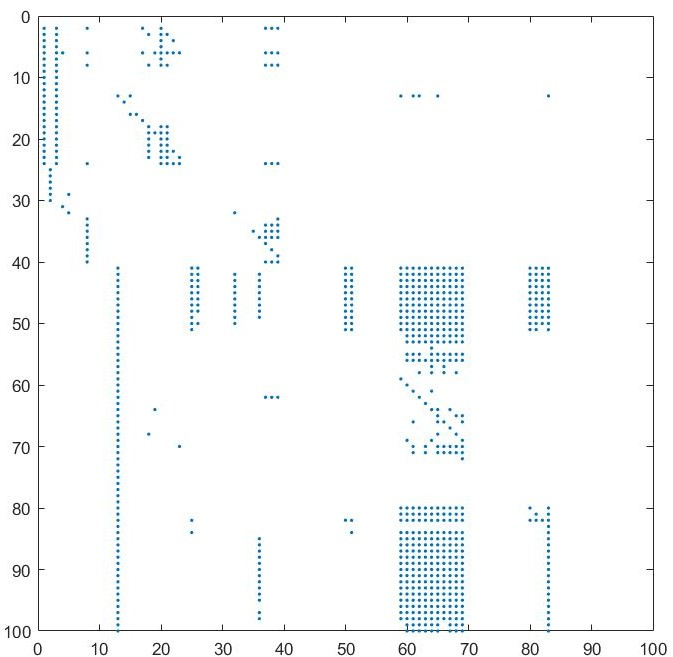
\includegraphics[width=0.6\textwidth]{multipl100.jpg}
    \caption{multiplayer.it sparse matrix with depth 100}
    
    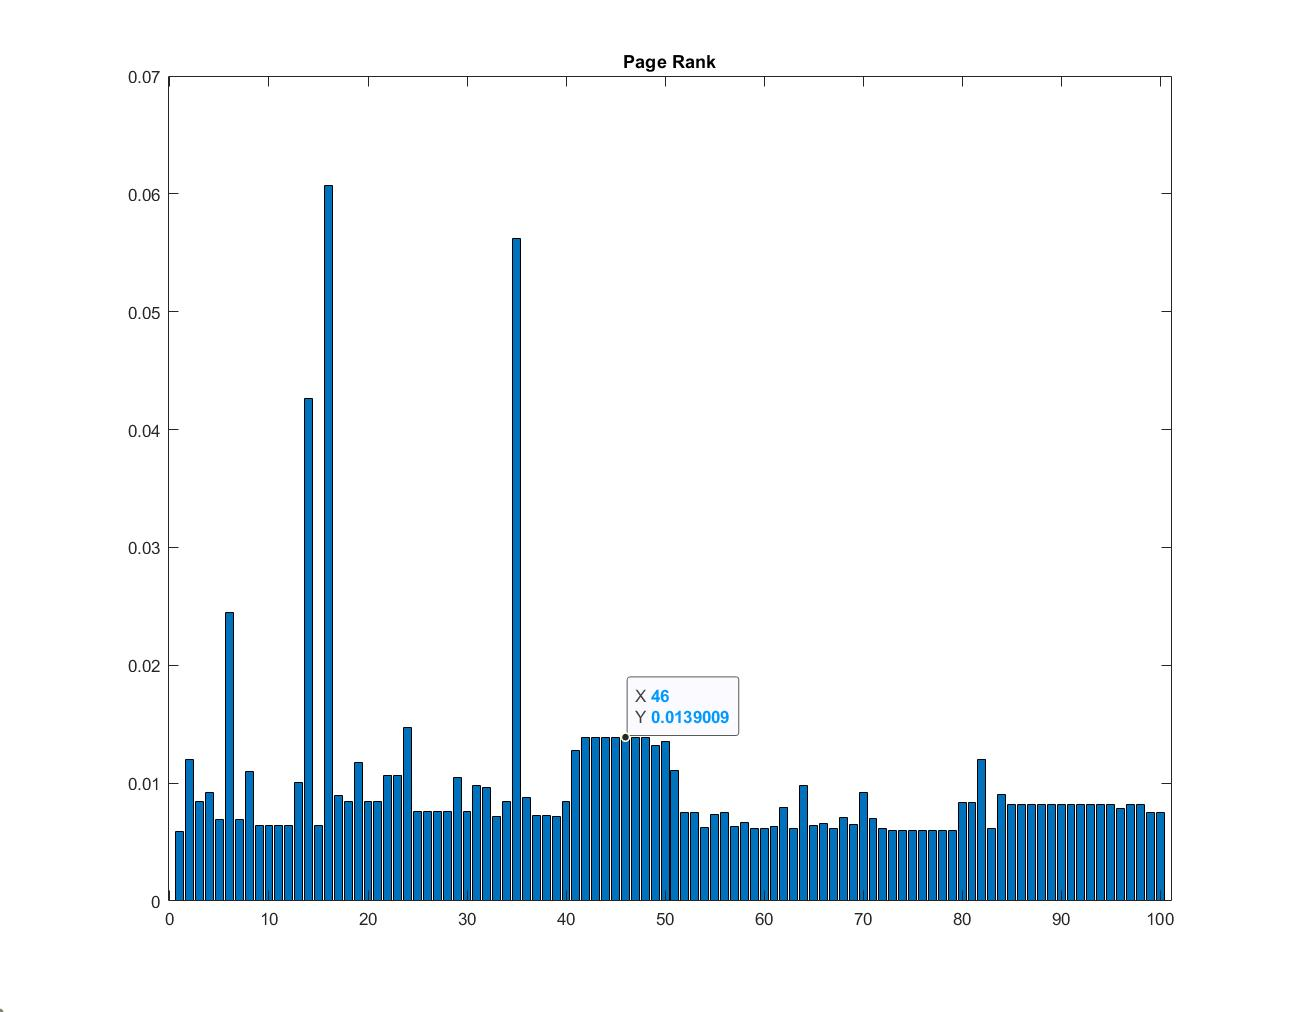
\includegraphics[width=0.7\textwidth]{multipl100PR.jpg}
    \caption{multiplayer.it Page Rank}
    \end{figure}

\newpage

\begin{center}
 \begin{tabular}{||c | c | c | c||} 
 \hline
 Page-Rank & In & Out & URL \\ [0.5ex] 
 \hline\hline
 0.0607 & 4 & 1 & https://www.instagram.com/multiplayer.it \\ 
 \hline
 0.0562 & 5 & 1 & https://t.me/multiplayershop \\
 \hline
 0.0426 & 3 & 1 & https://twitter.com/multiplayerit \\
 \hline
 0.0245 & 13 & 0 & https: \\
 \hline
 0.0147 & 10 & 0 & https://sb \\
 \hline
 0.0139 & 22 & 0 & https:\/\/live.adyen.com \\
 \hline
 0.0139 & 22 & 0 & https:\/\/integration-facebook.payu.in\\
 \hline
 0.0139 & 22 & 0 & https:\/\/facebook.payulatam.com \\
 \hline
 0.0139 & 22 & 0 & https:\/\/secure.payu.com \\
 \hline
 0.0139 & 22 & 0 & https:\/\/facebook.dlocal.com \\
 \hline
\end{tabular}
\end{center}

As we can see in Fig.1, we have two blocks in 40-55 x 60-70 and 80-100 x 60-70. These are all pages related to facebook.com. Even though the Facebook pages are heavily connected, they are not in the top 5 pages in the Page-rank analysis, that's because they have a low rank themselves. A small group of these Facebook pages appear after the top five having the same page-rank. This website is full of links to Facebook in order to be more visible in the social media. The two pages with best rank are the social media links of the website.

\newpage

    \item \href{http://www.fabiokaeppeli.ch/}{www.fabiokaeppeli.ch}:
    \begin{figure}[H]
    \centering
    
    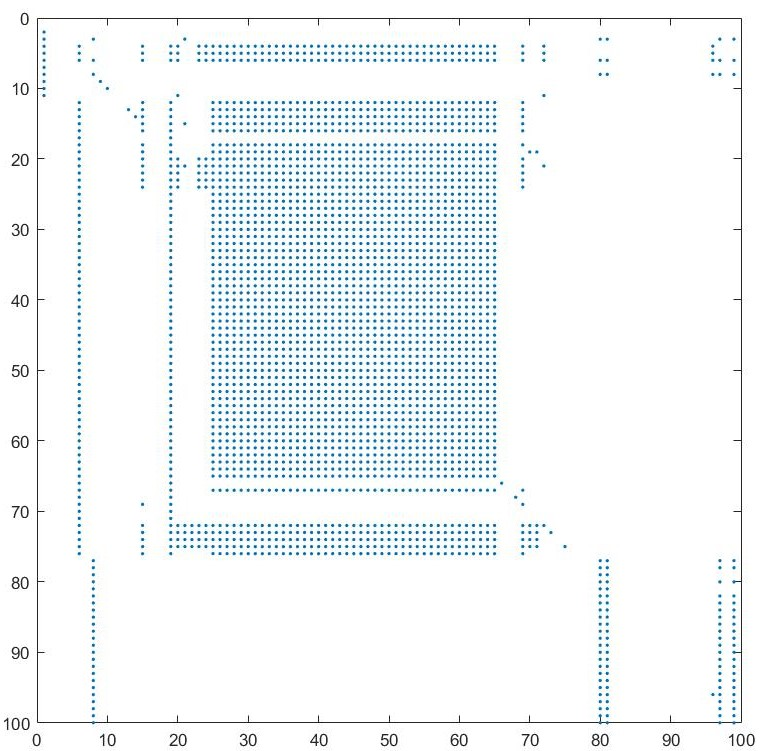
\includegraphics[width=0.6\textwidth]{fk100.jpg}
    \caption{fabiokaeppeli.ch sparse matrix with depth 100}
    
    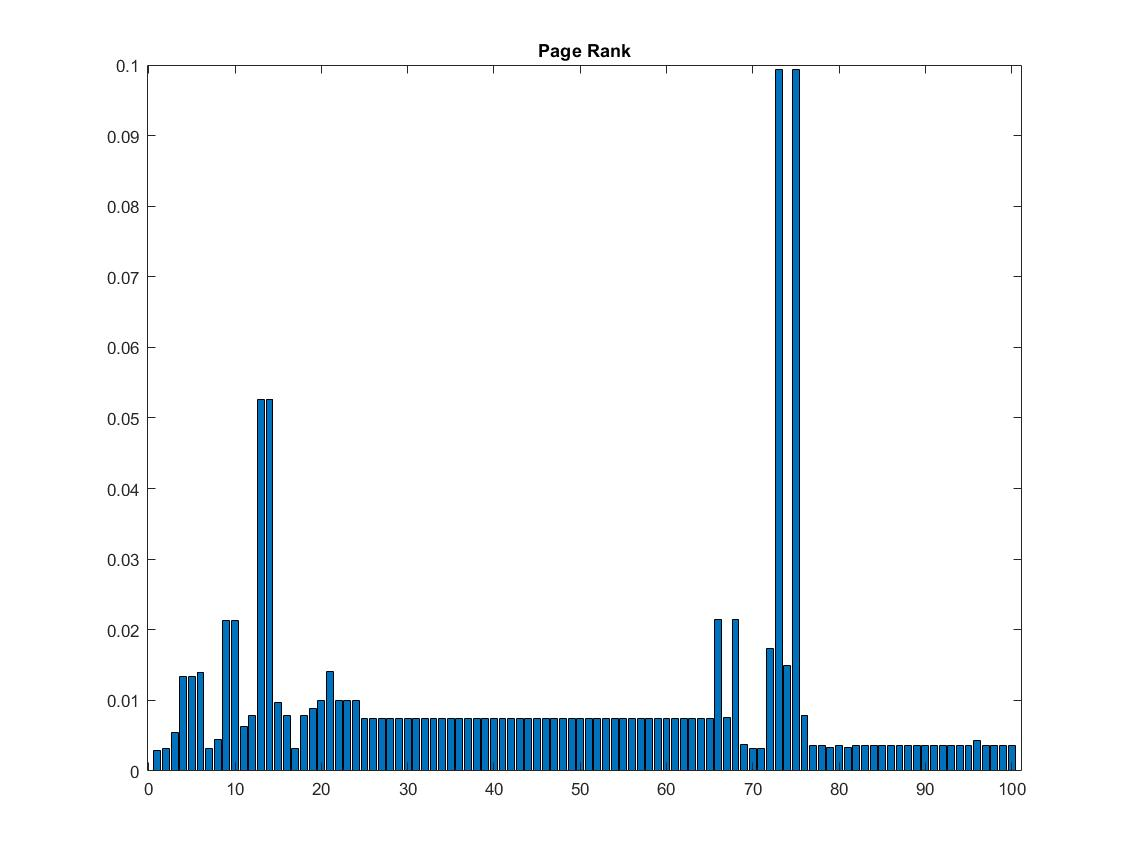
\includegraphics[width=0.7\textwidth]{fk100PR.jpg}
    \caption{fabiokaeppeli.ch Page Rank}
    \end{figure}

\newpage

\begin{center}
 \begin{tabular}{||c | c | c | c||} 
 \hline
 Page-Rank & In & Out & URL \\ [0.5ex] 
 \hline\hline
 0.0993 & 53 & 1 & https://publiccode.eu \\ 
 \hline
 0.0993 & 53 & 1 & https://www.facebook.com/WordPress \\
 \hline
 0.0527 & 46 & 1 & https://developer.wordpress.org/feed \\
 \hline
 0.0527 & 46 & 1 & https://developer.wordpress.org/comments/feed \\
 \hline
 0.0215 & 3 & 1 & https://github.com/WP-API/docs/edit/master/index.md \\
 \hline
 0.0215 & 3 & 1 & https://en.wikipedia.org/wiki/JSON\\
 \hline
 0.0212 & 2 & 1 & https://www.facebook.com/fabio.kaeppeli \\
 \hline
 0.0212 & 2 & 1 & https://twitter.com/fabiokep \\
 \hline
 0.0174 & 53 & 6 & https://wordpressfoundation.org/donate \\
 \hline
 0.0174 & 52 & 0 & https://twitter.com/WordPress \\
 \hline
\end{tabular}
\end{center}

This is a small website and it was made with WordPress, we can clearly see that from the surfer analysis. We can see a big block: links from 20 to 70 link to each other because they are part of developer.wordpress.org. Those links all have the same rank because, as said, they come from the same website, and the rank is quite low. We can see from the Page Rank that publicode.eu and the Facebook page of WordPress are on top with a very high score compared to the others. Also, a lot of pages have a link to themselves, since the diagonal has a lot of nonzero entries.

\newpage

    \item \href{https://stackexchange.com}{www.stackexchange.com}:
    \begin{figure}[H]
    \centering
    
    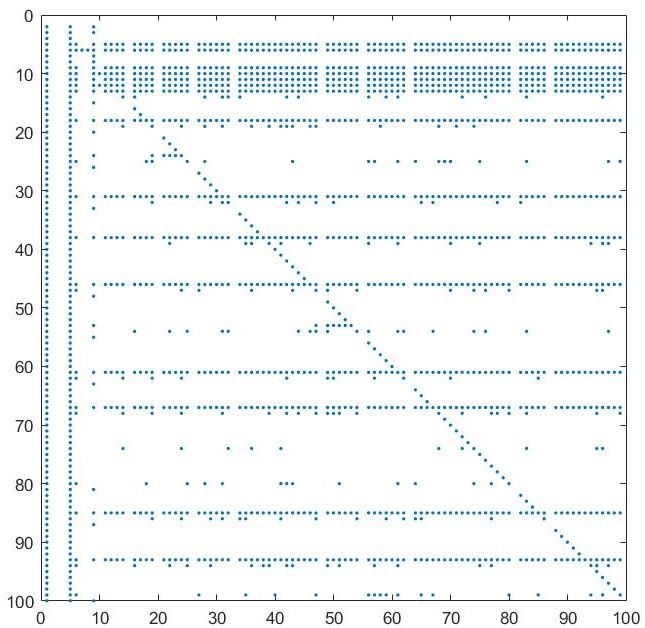
\includegraphics[width=0.6\textwidth]{se100.jpg}
    \caption{stackexchange.com sparse matrix with depth 100}
    
    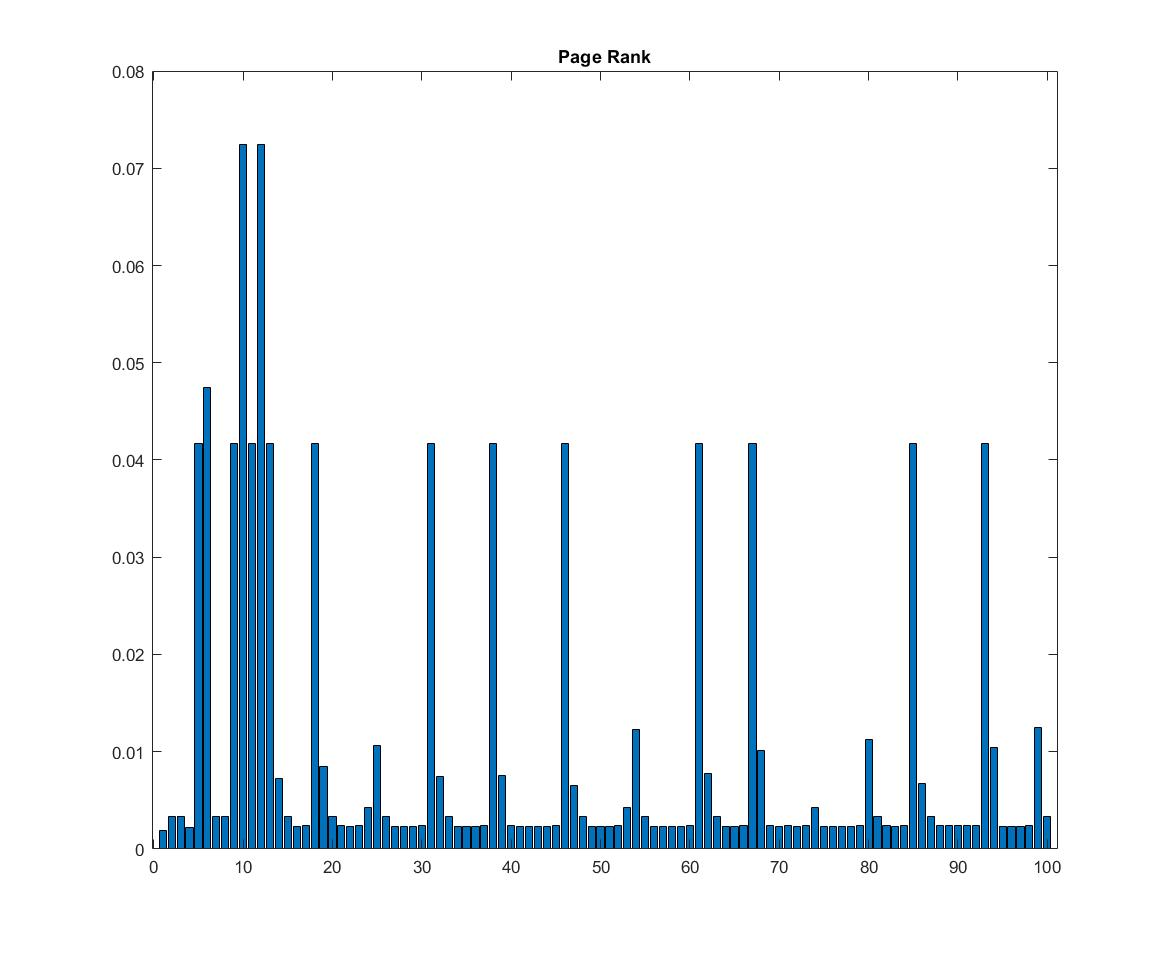
\includegraphics[width=0.7\textwidth]{se100PR.jpg}
    \caption{stackexchange.com Page Rank}
    \end{figure}

\newpage

\begin{center}
 \begin{tabular}{||c | c | c | c||} 
 \hline
 Page-Rank & In & Out & URL \\ [0.5ex] 
 \hline\hline
 0.0725 & 85 & 2 & https://stackoverflow.blog \\ 
 \hline
 0.0725 & 85 & 15 & https://stackoverflow.com/legal/privacy-policy \\
 \hline
 0.0474 & 86 & 22 & https://meta.stackexchange.com \\
 \hline
 0.0417 & 84 & 99 & https://stackexchange.com \\
 \hline
 0.0417 & 84 & 31 & https://stackexchange.com/sites \\
 \hline
 0.0417 & 84 & 15 & https://stackoverflow.com/legal/cookie-policy \\
 \hline
 0.0417 & 84 & 15 & https://stackoverflow.com/legal/terms-of-service/public \\
 \hline
 0.0417 & 84 & 17 & https://money.stackexchange.com \\
 \hline
 0.0417 & 84 & 22 & https://academia.stackexchange.com \\
 \hline
 0.0417 & 84 & 16 & https://worldbuilding.stackexchange.com \\
 \hline
\end{tabular}
\end{center}

This is a very big website. We can see from the surfer analysis that we have some patterns. The websites from 5 to 15 are linked by almost every page and have a fairly high Page Rank because they come from stackoverflow.com and stackexchange.com (stackexchange is the network of websites and stackoverflow is one of those). Almost every
page has a link to itself, since the diagonal is almost non zero everywhere. We can also see that the pages that are linked a lot for example pages 31, 38, 46, 61,...) also have a fairly high rank and it is the same.
 
\end{itemize}

\newpage

\subsection{Connectivity matrix and subcliques [10 points]}
The near cliques that we can see are caused by links that share the same domain.

\begin{itemize}
    \item  Around index 80: \href{http://www.baug.ethz.ch}{ www.baug.ethz.ch}
    \item  Around index 120: \href{http://www.mat.ethz.ch}{www.mat.ethz.ch}
    \item  Around index 170: \href{http://www.mavt.ethz.ch}{www.mavt.ethz.ch}
    \item  Around index 205: \href{http://www.biol.ethz.ch}{www.biol.ethz.ch}
    \item  Around index 230: \href{http://www.chab.ethz.ch}{www.chab.ethz.ch}
    \item  Around index 270: \href{http://www.math.ethz.ch}{www.math.ethz.ch}
    \item  Around index 325: \href{http://www.erdw.ethz.ch}{www.erdw.ethz.ch}
    \item  Around index 365: \href{http://www.usys.ethz.ch}{www.usys.ethz.ch}
    \item  Around index 400: \href{http://www.mtec.ethz.ch}{www.mtec.ethz.ch}
    \item  Around index 445: \href{http://www.gess.ethz.ch}{www.gess.ethz.ch}
    \item  Around index 495: \href{http://www.bilanz.ch}{www.bilanz.ch}
\end{itemize}

\subsection{Connectivity matrix and disjoint subgraphs [10 points]}
\begin{enumerate}
    \item The connectivity matrix G:
    \[
    \begin{bmatrix}
    \centering
    0 & 0 & 0 & 1 & 0 & 0\\
    1 & 0 & 0 & 0 & 0 & 0\\
    1 & 1 & 0 & 0 & 0 & 0\\
    0 & 1 & 1 & 0 & 0 & 0\\
    0 & 0 & 0 & 0 & 0 & 1\\
    0 & 0 & 0 & 0 & 1 & 0\\
    \end{bmatrix}
    \]

    \begin{figure}[H]
    \centering
    
    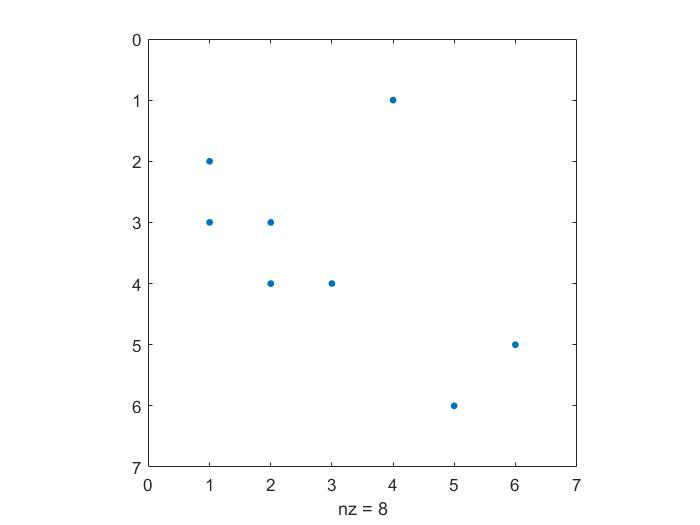
\includegraphics[width=0.7\textwidth]{myG.jpg}
    \end{figure}
    
    \newpage
    
    \item Page ranks with default p = 0.85:
    
    \begin{center}
         \begin{tabular}{||c | c | c | c||} 
         \hline
         Page-Rank & In & Out & URL \\ [0.5ex] 
         \hline\hline
         0.2037 & 2 & 1 & http://www.delta.com \\ 
         \hline
         0.1981 & 1 & 2 & http://www.alpha.com \\
         \hline
         0.1667 & 1 & 1 & http://www.rho.com \\
         \hline
         0.1667 & 1 & 1 & http://www.sigma.com \\
         \hline
         0.1556 & 2 & 1 & http://www.gamma.com \\
         \hline
         0.1092 & 1 & 2 & http://www.beta.com \\
         \hline
        \end{tabular}
        \end{center}
    
    \begin{figure}[H]
    \centering
    
    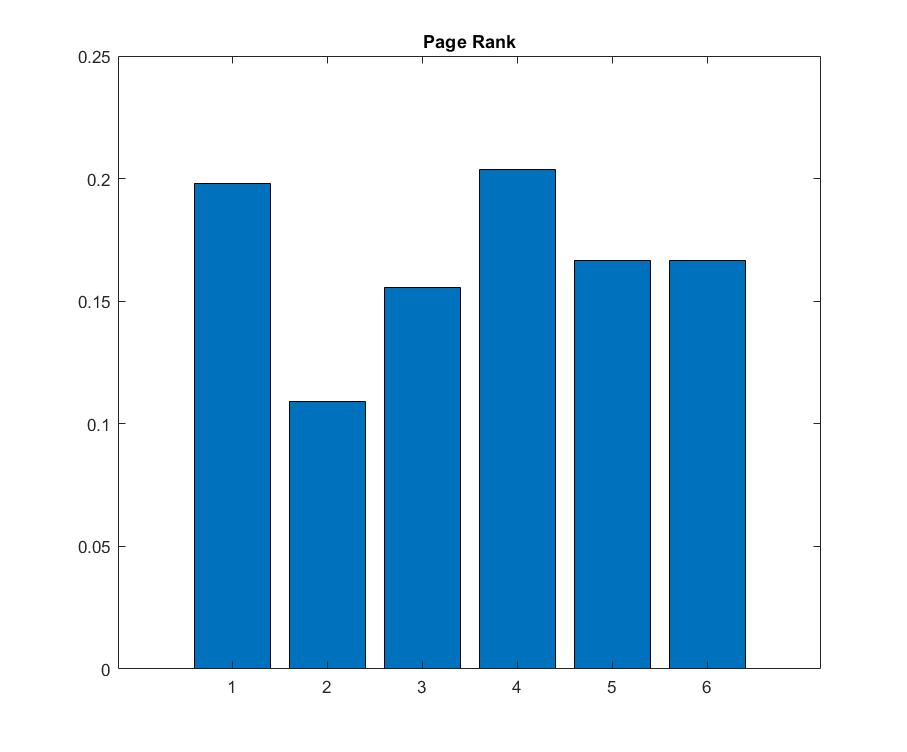
\includegraphics[width=0.7\textwidth]{ex4_85.jpg}
    \end{figure}
    
    \item Let's try using pagerank with p = 0.99999:
    
        \begin{center}
         \begin{tabular}{||c | c | c | c||} 
         \hline
         Page-Rank & In & Out & URL \\ [0.5ex] 
         \hline\hline
         0.2051 & 2 & 1 & http://www.delta.com \\ 
         \hline
         0.2051 & 1 & 2 & http://www.alpha.com \\
         \hline
         0.1667 & 1 & 1 & http://www.rho.com \\
         \hline
         0.1667 & 1 & 1 & http://www.sigma.com \\
         \hline
         0.1538 & 2 & 1 & http://www.gamma.com \\
         \hline
         0.1026 & 1 & 2 & http://www.beta.com \\
         \hline
        \end{tabular}
        \end{center}
    
    \begin{figure}[H]
    \centering
    
    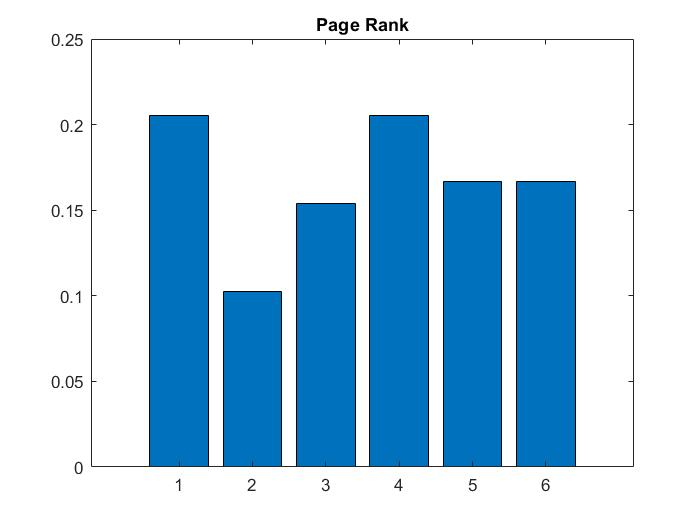
\includegraphics[width=0.7\textwidth]{ex4_9999.jpg}
    \end{figure}
    
    As we can see, alpha has the same rank as delta. That's because with probability \( p \rightarrow 1 \), the pagerank algorithm doesn’t let you choose another page randomly:
    
    \[ \delta = \frac{1 - p}{n} \]
    \[ \delta =\lim_{p\rightarrow 1} \frac{1 - p}{n} = 0, \]
    with $\delta$ the probability that a particular random page is chosen.
    
\end{enumerate}


\subsection{PageRanks by solving a sparse linear system [50 points]}

\begin{enumerate}

    \item \checkmark
    
    \item We want $x$ with $x = Ax$. Knowing that the eigenvalue is $\lambda = 1$, we use as a stop criterion
    \[|| Ax^k - x^k ||\leq \epsilon\] with $\epsilon$ the machine precision. With \( A^k x_0 = x^k \) we have \( Ax^k = AA^k x_0 = A^{k+1}x_0 \) and : \[|| x - old\_x ||\leq \epsilon.\]  
    
    \begin{figure}[H]
    \centering
    
    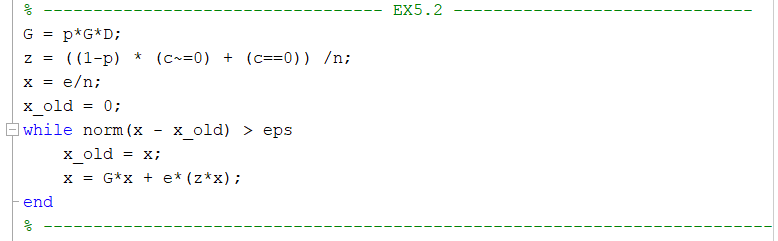
\includegraphics[width=0.9\textwidth]{ex5_2.png}
    \end{figure}
    
    \item Having in mind that our dominant $\lambda$ is equal to one, we have that setting $\alpha = 1$ gives us the fastest convergence, likely much faster than the Power method where more than one eigenvalue is dominant. As we go further away from 1 ($\alpha = 0.9$ and $\alpha = 0.8$) the convergence slows down.\\
    In order to prevent a division by zero we can use Gaussian elimination with partial pivoting, this always produces a solution with a small residual that prevents any exact zero divisions. Another way can be to approximate $\alpha = 1$ with something like $\alpha = 0.9999$, preventing some diagonal element from being exactly 0.
    
    \item All three algorithms give the same result:
    \begin{figure}[H]
    \centering
    
    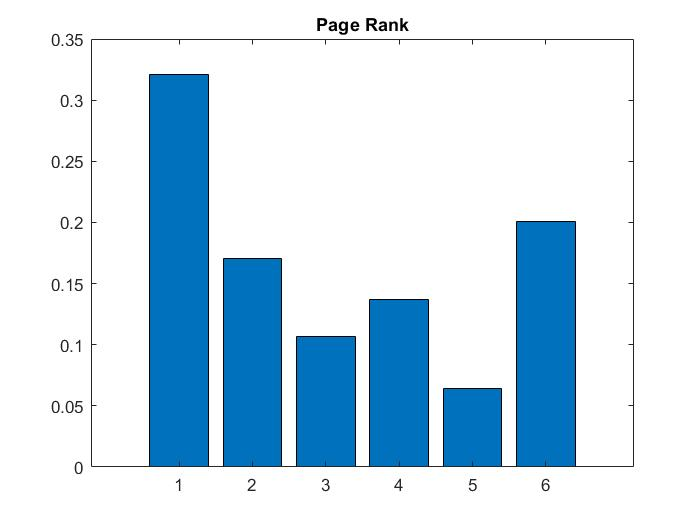
\includegraphics[width=0.6\textwidth]{ex5_4_0.jpg}
    \caption{pagerank.m}
    \end{figure}
    \begin{figure}[H]
    \centering
    
    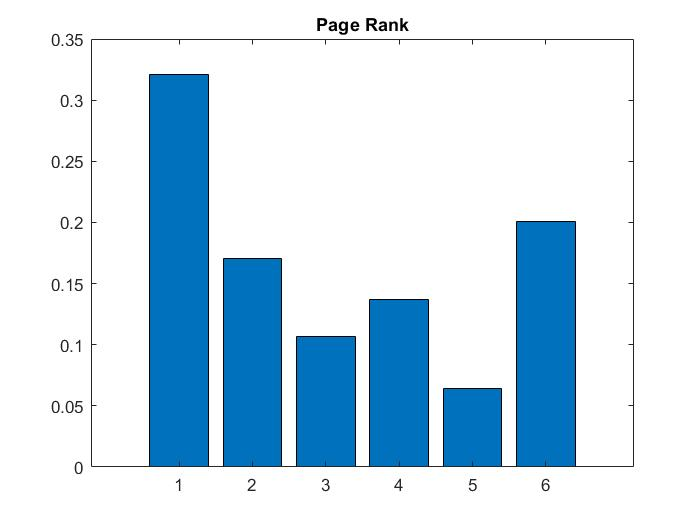
\includegraphics[width=0.6\textwidth]{ex5_4_0.jpg}
    \caption{pagerank1.m}
    \end{figure}
    \begin{figure}[H]
    \centering
    
    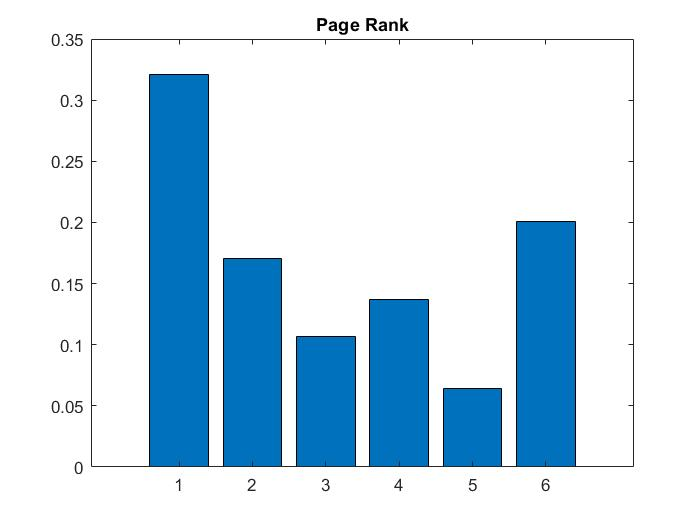
\includegraphics[width=0.6\textwidth]{ex5_4_2.jpg}
    \caption{pagerank2.m}
    \end{figure}
    With the following PageRanks:
    \begin{center}
         \begin{tabular}{||c | c | c | c||} 
         \hline
         Page-Rank & In & Out & URL \\ [0.5ex] 
         \hline\hline
          0.3210  & 2 & 2 & http://www.alpha.com \\ 
         \hline
         0.2007 & 2 & 1 & http://www.sigma.com \\
         \hline
         0.1705 & 1 & 2 & http://www.beta.com  \\
         \hline
         0.1368 & 2 & 1 & http://www.delta.com \\
         \hline
         0.1066 & 1 & 3 & http://www.gamma.com \\
         \hline
         0.0643 & 1 & 0 & http://www.rho.com \\
         \hline
        \end{tabular}
        \end{center}
        
    \item Also for figure 5 the three algorithms produce the same result:
    \begin{center}
         \begin{tabular}{||c | c | c | c||} 
         \hline
         Page-Rank & In & Out & URL \\ [0.5ex] 
         \hline\hline
         0.2037 & 2 & 1 & http://www.delta.com \\ 
         \hline
         0.1981 & 1 & 2 & http://www.alpha.com \\
         \hline
         0.1667 & 1 & 1 & http://www.rho.com \\
         \hline
         0.1667 & 1 & 1 & http://www.sigma.com \\
         \hline
         0.1556 & 2 & 1 & http://www.gamma.com \\
         \hline
         0.1092 & 1 & 2 & http://www.beta.com \\
         \hline
        \end{tabular}
        \end{center}
    
    There is some difference between task 5.5 and 5.4:
    \begin{center}
         \begin{tabular}{||c | c | c||} 
         \hline
         Page-Rank - Fig5 & Page-Rank - Fig1 & URL \\ [0.5ex] 
         \hline\hline
         0.1981 & 0.3210 & http://www.alpha.com \\
         \hline
         0.1092 & 0.1705 & http://www.beta.com \\
         \hline
         0.1556 & 0.1066 & http://www.gamma.com \\
         \hline
         0.2037 & 0.1368 & http://www.delta.com \\ 
         \hline
         0.1667 & 0.0643 & http://www.rho.com \\
         \hline
         0.1667 & 0.2007 & http://www.sigma.com \\
         \hline
        \end{tabular}
        \end{center}
    We can clearly see that two different graphs produce very different Pageranks. For example, alpha loses one incoming link and goes from first to second place. We can conclude that even slightly changing the links between the pages can have a huge impact in the Pageranks.
    
    \item For the website multiplayer.it the three algorithms produced the same result as in exercise 2. pagerank1.m required 168 iterations. pagerank2.m required 2 iterations.\\ \\
    For the website fabiokaeppeli.ch the three algorithms produced the same result as in exercise 2. pagerank1.m required 126 iterations. pagerank2.m required 2 iterations.\\ \\
    For the website stackexchange.com the three algorithms produced the same result as in exercise 2. pagerank1.m required 38 iterations. pagerank2.m required 2 iterations.\\\\\\
    The advantage of the power method is that we exploit the sparsity matrix without actually forming a Markov matrix. This way we don’t have to solve a linear system ($\mathcal{O}(n^3)$ and for real network applications this is simply unfeasible) but just the addition of two multiplication of sparse matrices and a vector ($\mathcal{O}(n^2)$) which is  repeated until the stop criterion is reached. The ratio of convergence is given by $|\frac{\lambda_2}{\lambda_1}|$, if $\lambda_2$ is close in magnitude to $\lambda_1$ the convergence may be extremely low. In pagerank2 we implemented the inverse method that gives much faster convergence (as we can see from the previous results) at the cost of having to solve a linear system at each iteration. Even if pagerank2 needs to compute a linear system as in the original pagerank, using the shift and invert technique and with $\alpha$ is very close to $\lambda_1$, convergence of pagerank2 is expected to be very fast and much fuster that pagerank and pagerank1 (only for smaller problems).
    
    
    
    
    
\end{enumerate}
\end{document}
